\documentclass[12pt,a4paper]{article}

\usepackage{ucs}
\usepackage[utf8x]{inputenc}
\usepackage[T2A]{fontenc}
\usepackage[russian]{babel}
\usepackage{amsthm}
\usepackage{amsmath}
\usepackage{amssymb}
\usepackage{graphicx}
\usepackage{float}
\usepackage{clrscode}
\usepackage{tocloft}
\frenchspacing

\theoremstyle{plain}
\newtheorem*{thm}{Теорема}
\newtheorem*{lem}{Лемма}
\theoremstyle{definition}
\newtheorem*{defn}{Определение}

%\setlength{\headheight}{0pt}
%\setlength{\headsep}{0pt}
%\setlength{\topmargin}{-1.0cm}
%\setlength{\textheight}{25.0cm}
%\setlength{\textwidth}{17.6cm}
%\setlength{\oddsidemargin}{0cm}
%\setlength{\evensidemargin}{0pt}
%\setlength{\marginparsep}{0pt}
%\setlength{\marginparpush}{0pt}
%\parindent=15mm
%\setlength{\leftmargini}{\parindent}
%\addtolength{\leftmargini}{4mm}
%\setlength{\headheight}{0pt}
%\setlength{\headsep}{0pt}


\begin{document}

\title{Конспект вопросов по компьютерной алгебре. Первый семестр. 2010.}
\author{Преподаватель: Васильев Николай Николаевич}
\date{}
\maketitle
\thispagestyle{empty}

\pagebreak

\renewcommand{\cftsecleader}{\cftdotfill{\cftsubsecdotsep}}
\tableofcontents

\pagebreak

\section{Группа, подгруппа, гомоморфизм групп. Ядро и образ гомоморфизма.}

\begin{defn}
   \(<G, *, e>\) - группа, 
   \(*: G \times G \rightarrow G, e \in G \) 
   \begin{enumerate}       
     \item \( \forall a, b, c \in G \; (ab)c=a(bc) \)
     \item \( \forall g \in G \; eg = ge = g \)
     \item \( \forall g \in G \; \exists g^{-1} \in G \; gg^{-1} = g^{-1}g = e \)
   \end{enumerate}
   Если \( \forall a, b \in G \; ab = ba \) то группу называют \emph{абелевой} 
\end{defn}

\begin{thm}
  \( \exists ! e \in G \; eg = ge = g \)
\end{thm}

\begin{defn}
  \( G \) - группа, тогда \( H \subset G \) называют \emph{подгруппой}, если 
  \begin{enumerate}
    \item \( e \in H \)
    \item \( \forall h_1, h_2 \in H \; h_{1}h_{2} \in H \; | \; HH \subset H \)
    \item \( \forall h \in H \; h^{-1} \in H \; | \; H^{-1} \subset H \)
  \end{enumerate}
\end{defn}

\begin{defn}
  \( G, W \) - группы. \newline
  \( f: G \rightarrow W \) называют \emph{гомоморфизмом (групп)}, если \( \forall g_1, g_2 \in G \; f(g_{1}g_2) = f(g_1) * f(g_2) \)
\end{defn}

\begin{thm}
  \( f: G \rightarrow W \) - гомоморфизм \newline
  \( f(e_G) = e_W \)
\end{thm}

\begin{defn}
    \( f: G \rightarrow W \) - гомоморфизм, тогда \newline
    \( ker f = \{ g \in G | f(g) = e_W \} \) - называют \emph{ядром гомоморфизма f}
\end{defn}

\begin{thm}
  \( ker f \) - подгруппа \( G \)
\end{thm}

\begin{defn}
   \( f: G \rightarrow W \) - гомоморфизм, тогда \newline
   \( Im f = \{ w \in W | \exists g \in G \; f(g) = w \} \) - называют \emph{образом гомоморфизма f}
\end{defn}

\section{Мономорфизмы, эпиморфизмы и изоморфизмы. Понятие нормального делителя (нормальной подгруппы). Факторгруппа.}

\begin{defn}
  Сюръективный гомоморфизм - \emph{эпиморфизм}. \newline
  Инъективный гомоморфизм - \emph{мономорфизм}. \newline
  Биективный гомоморфизм - \emph{изоморфизм}. \newline
  Изоморфизм $ f: G \rightarrow G $ - \emph{автоморфизм}. \newline
\end{defn}

Пусть $ H \subset G $. Введем отношение эквивалентности $ \sim $ соответствующее подгруппе. $ g_1, g_2 \in G $. $ g_1 \sim g_2 $, если $ g_{1}g_{2}^{-1} \in H $

\begin{defn}
  $  \overset{\sim}{g} = \{ k \in G | k \sim g\} $ - \emph{класс эквивалентности элемента, левый смежный класс} $g$ \newline
  Обозначение: $ Hg $
\end{defn}

\begin{defn}
  $ G/H $ - \emph{фактормножество}, множество смежных классов. $ G/H = \{ \overset{\sim}{g} \; | \; \overset{\sim}{g} = Hg \} $ 
\end{defn}

Заметим, что в случае некоммутативной группы можно ввести правые смежные классы $ gH $.

\begin{thm}
  Если $ gH = Hg $, то $ G/H $ - группа и называется факторгруппой.
\end{thm}

\begin{proof}  
  Введем умножение: $ \forall g_{1}H, g_{2}H \in G/H \; (g_{1}H)(g_{2}H){\buildrel{def}\over{=}}g_{1}g_{2}H $.
  Проверим корректность умножения: пусть $ g_1' \sim g_1, g_2' \sim g_2 $. Тогда
  $ g_1' = g_{1}h_1, g_2' = g_{2}h_2 $, а значит $ g_{1}'g_{2}'= g_{1}h_{1}g_{2}h_{2} = g_{1}g_{2}h_{1}h_{2} $. 
  То есть $ g_{1}'g_{2}'H = g_{1}g_{2}H $. \newline
  Теперь проверим свойства умножения: 
  \begin{enumerate}
    \item $ eHgH = gH $
    \item $ g_{1}Hg_{2}Hg_{3}H = g_{1}g_{2}g_{3}H $
    \item $ gHg^{-1}H = eH $
  \end{enumerate}
\end{proof}

\begin{defn}
  $H \subset G$ назовем \emph{нормальной подгруппой}, если $ \forall g \in G \; gH = Hg $ или $ gHg^{-1} = H $ или $ ghg^{-1} \in H $  
  \newline Обозначение: $H \triangleleft G$
\end{defn}

\begin{thm}
  $ G $ - абелева группа, тогда $ \forall H \subset G $ - нормальная.
\end{thm}

\pagebreak

\begin{thm}
  Ядра гомоморфизмов и только они суть нормальные подгруппы.
\end{thm}
\begin{proof}
  Сперва докажем, что если $ f: G \rightarrow W $ - гомоморфизм, то $ ker f \triangleleft G $. 
  $ g \in G, h \in ker f $, тогда $ f(ghg^{-1}) = f(g)f(h)f(g^{-1}) = f(g)f(g)^{-1} = e_W $. \newline
  Теперь покажем, что $ \forall H \triangleleft G \; \exists f $ - гомоморфизм и $ ker f = H $.
  Введем $ \pi_{H} : G \rightarrow G/H $ - канонической гомоморфизм. Пусть $ g \in G, h \in H $ 
  тогда $\pi_{H}(g) = gH, \pi_{H}(h) = hH = H $. Следовательно $ ker \pi_{H} = H $.
\end{proof}

Порой пишут: $ \{e\} \subset H \triangleleft G \overset{\pi_{H}}{\rightarrow} G/H $ 






\section{Характеризация мономорфизмов в терминах ядра. Основная теорема о гомоморфизме.}

\begin{thm}
$ \phi $ - мономорфизм $ \Leftrightarrow ker \phi = \{e\} $
\end{thm}
\begin{proof}
  $ [\Rightarrow] $ Пусть $ \exists g \ne e $ $ \phi(g) = e $. Но $ \phi(e) = e $. Таким образом $ g \ne e, \phi(g) = \phi(e) $. 
  Противоречие инъективности. \newline
  $ [\Leftarrow] $ Пусть $ \exists g_{1} \ne g_{2}, \phi(g_{1}) = \phi(g_{2}) $. Тогда $ \phi(g_{1})\phi(g_{2})^{-1} = e $,
  а это значит, что $ g_{1}g_{2}^{-1} \ne e $ и $ g_{1}g_{2}^{-1} \in ker f $. Противоречие тривиальности ядра. 
\end{proof}

\begin{thm}
  $ G/ker f \buildrel{\sim}\over{=} Im f $
\end{thm}
\begin{proof}
  Пусть $ \phi : X \rightarrow Y $. Введем отношение эквивалентности: $ x_1 \sim x_2 $, если $ \phi(x_1) = \phi(x_2) $. 
  Рассмотрим $ \tau : X/\!\!\!\sim  $ $ \rightarrow Im \, \phi, $ $ \tau(\overset\sim{x}) = \phi(x). $ \newline
  $ \tau $ - инъекция. Действительно, если $ \overset\sim{x_1} \ne \overset\sim{x_2} $, то $ x_1 $ не эквивалентно $ x_2 $
  и значит $ \phi(x_1) \ne \phi(x_2) $. \newline
  $ \tau $ - сюръекция. Действительно $ \forall y \in Im \, \phi $ $ \exists x \; \phi(x) = y $ и 
  $ \overset\sim{x} : \tau(\overset\sim{x}) = y $. Таким образом изоморфизм установлен. \newline
  Теперь пусть $ f : G \rightarrow W $ - гомоморфизм. $ g_1 \sim g_2 $, если $ f(g_1) = f(g_2) $, или 
  $ f(g_1)f(g_2)^{-1} = e, f(g_1g_2^{-1}) = e $ это означает, что $ g_1g_2^{-1} \in ker f $. То есть отношение $ \sim $
  совпадает с отношением эквивалентности порождаемым $ ker f \triangleleft G $. Можно записать
  $ G/ker f \buildrel{\sim}\over{=} Im f $.
\end{proof}




\section{Группа подстановок (симметрическая группа). Четные и нечетные подстановки. 
Теорема о том, что всякая группа есть подгруппа симметричской группы (для конечных групп).}

\begin{defn} 
  \emph{Симметрической группой} $ S_{X} $ множества $ X $ называется группа автоморфизмов $ X \rightarrow X $
  относительно операции композиции и нейтрального элемента $ id_{X} : \forall x \in X, id_{X}(x) = x $. \newline
  Если $ X = \{1, 2, \cdots, n \} $, то симметричскую группу называют группой подстановок и обозначают $ S_{n} $. 
\end{defn}

Группа подстановок $ S_{n} $ допускает следующее копредставление: \newline

Образующие: \newline
$ \sigma_{1}, \sigma_{2}, \cdots ,\sigma_{n-1} $ \newline

Соотношения: \newline
$ \sigma_{i}^{2} = 1 $ \newline
$ \sigma_{i}\sigma_{j} = \sigma_{j}\sigma_{i} $, если $ |i - j| > 1 $ \newline
$ \sigma_{i}\sigma_{i+1}\sigma_{i} = \sigma_{i+1}\sigma_{i}\sigma_{i+1} $ \newline

Вообще, образующие в указанном копредставлении являются \emph{транспозициями}, то есть это такие подстановки,
которые меняют два соседних элемента местами, а остальные элементы оставляют на месте.

\begin{defn}
  Подстановка называется \emph{четной}, если она представляется в виде произведения четного числа транспозиций и 
  \emph{нечетной} в противном случае.
\end{defn}

\begin{thm}
  Любая группа - подгруппа симметрической группы.
\end{thm}
\begin{proof}
  Необходимо сопоставить каждому элементу $ g \in G $ некоторую биекцию $ G \rightarrow G $, тем самым получив вложение $ G \subset S_{G} $.
  Рассмотрим $ i_{g} : G \rightarrow G, \forall s \in G \; i_{G}(s) = gs $. 
  Осталось проверить свойства: $ i_{a} \circ i_{b} = a(bs) = (ab)s = i_{ab}, \; i_{g} \circ i_{g^{-1}} = g(g^{-1}s) = es = i_{e} $.
\end{proof}


\section{Левые классы смежности по подгруппе (см. вопрос 2). Индекс подгруппы. Теорема об индексе.}

\begin{defn}
  $ H \subset G $ \newline
  $ [G:H] = \#(G/H) $ - \emph{индекс} подгруппы. То есть индекс подгруппы это количество смежных классов. \newline
  $ \#G $ - \emph{порядок}, \emph{мощность} группы. 
\end{defn}

Замечание: индекс тривиальной подгруппы - порядок группы.

\begin{thm}[Теорема об индексе]
  $ K \subset H \subset G $, \newline тогда $ [G:K] = [G:H][H:K] $
\end{thm}
\begin{proof}
  $ G = \overset{[G:H]}{\underset{i=1}{\bigcup}} g_{i}H $ при этом $ g_{i}H \ne g_{j}H, i \ne j $. 
  Аналогично $ H = \overset{[H:K]}{\underset{j=1}\bigcup} h_{j}K $ при этом $ h_{i}K \ne h_{j}K, i \ne j $. 
  Запишем $ G = \underset{i, j}\bigcup \, g_{i}h_{j}K $. \newline
  Теперь достаточно проверить, что $ g_{i}h_{j}K $ представляют все различные классы смежности по $ K $.
  Пусть $ g_{i}h_{j}K = g_{l}h_{m}K $. Умножим на $ H $, получим $ g_{i}h_{j}KH = g_{l}h_{m}KH $, и далее
  $ g_{i}h_{j}H = g_{l}h_{m}H \Rightarrow  g_{i}H = g_{l}H \Rightarrow i = l $. Вернемся к исходному равенству
  $ g_{i}h_{j}K = g_{i}h_{m}K \Rightarrow h_{j}K = h_{m}K \Rightarrow j = m $. То есть все классы различны. \newline
  Возьмем $ gK $. Ясно, что $ g = g_{i}h, h \in H $ и $ h = h_{m}k, k \in K $. Имеем 
  $ g = g_{i}h_{m}k, g \in g_{i}h_{m}K $. Теперь понятно, что исходное представление $ G $ представляло все классы
  смежности по $ K $.
\end{proof}

Следствия:

\begin{enumerate}
  \item Порядок подгруппы всегда делитель порядка группы. \newline
    Пусть $ K = \{e\} $, по теореме об индексе $ \#G = \#(G/H)\#H $
  \item $ \forall G : \#G = p, p \in \mathbb{P} $ - циклическая группа порядка p \newline
    Рассмотрим $ G : \#G = p, p \in \mathbb{P} $. Рассмотрим $ H \subset G $ - циклическая подгруппа,
    порожденная $ g \ne e $. Ясно, что $ \#H \ge 2 $. Но $ \#H $ делитель $ \#G = p $, а значит
    $ \#H = p = \# G $. Также из этого следует $ \forall G : \#G = p, p \in \mathbb{P} \;\;\;\; 
    G \overset\sim{=} \mathbb{Z}/p\mathbb{Z} $
\end{enumerate}

\section{Действие группы на множестве. Орбиты. Разбиение множества на орбиты и формула орбит. Стабилизатор.}

\begin{defn}
Под действием группы $G$ на множестве $X$ понимается: $s: G \times X \rightarrow X$ со свойствами:
\begin{enumerate}
  \item $s(g_1, s(g_2, x)) = s(g_1 g_2, x)$
  \item $s(e, x)) = x$
\end{enumerate}
\end{defn}

\vspace{0.5cm}
$x \mapsto s(g, x)$ обозначим как $i_g$. Обратное действие - $s^{-1}(g, x) = s(g^{-1}, x)$. \\
\par Обозначим $s(g, x) = g \cdot x, т.е.:$
\begin{enumerate}
 \item $g_1(g_2x) = (g_1g_2)x$
 \item $ex = x$
\end{enumerate}

\begin{defn}
Орбитой точки $x \in X$ назовем множество $Gx = \{ s(g, x) | g \in G \}$
\end{defn}

\begin{lem}
Множество орбит - разбиение множества $X$. Орбиты либо совпадают, либо не пересекаются.
\end{lem}
\begin{proof}
Пусть $y \in G{x_1} \bigcap G{x_2}$. Это значит, что $ \exists g_1, g_2: y = g_1x_1 = g_2x_2$.
Рассмотрим элемент $\widetilde{y} = gx_1$ из орбиты $G{x_1}$. Но $\widetilde{y} = gg^{-1}_1y = gg^{-1}_1g_2x_2$. 
Значит $\widetilde{y}$ из орбиты $G{x_2}$. Следовательно орбиты совпадают.
\end{proof}

\begin{defn}
Назовем стабилизатором точки $x \in X$ множество $S_x \subset G: S_x = \{g \in G | gx = x \}$.
\end{defn}

\begin{lem}
Стабилизаторы различных точек сопряжены в одной. $x$ и $x_1$ - точки одной орбиты,
тогда $\exists g: S_x = gS_{x_1}g^{-1}$.
\end{lem}
\begin{proof}
$x_1 = gx$ - т.к. они с одной орбиты. $x = g^{-1}x_1$. Рассмотрим $w \in S_x: wx = x$. 
\begin{center}
$wg^{-1}x_1 = g^{-1}x_1$\\
$gwg^{-1}x_1 = x_1$\\
$gwg^{-1} \in S_{x_1}$
\end{center}
\end{proof}

Орбиты будем обозначать $O_x = Gx$.

\begin{thm}
$|O_x| = \#(O_x) = [G : S_x], \forall x \in X$
\end{thm}
\begin{proof}
Введем эквивалентность: $g_1 \sim g_2 {\buildrel{def}\over{\Leftrightarrow}} g_1x = g_2x
\Leftrightarrow g^{-1}_1g_2x = x \Leftrightarrow g^{-1}_1g_2 \in S_x$. Таким образом, 2 элемента эквивалентны, если они
переводят элемент $x$ в один и тот же элемент орбиты. 2 элемента из разных классов эквивалентности переводят элемент $x$ в
разные элементы орбиты. Разобьем всю группу на классы эквивалентности $G/S_x$. Отсюда $\#(O_x) = [G : S_x]$.
\end{proof}

\begin{thm}[Формула орбит]
$X = {\underset{x \in Orb(X)}{\bigcup}}O_x$, ($x \in Orb(x)$ - берем по одному представителю со всех орбит) \\
$|X| = {\underset{x \in Orb(X)}{\sum}}|O_x| = {\underset{x \in Orb(X)}{\sum}}[G : S_x]$
\end{thm}



\section{Действие группы на себе сопряжениями. Сопряженные элементы. Классы сопряженности. Формула классов.}

Для всякого $x \in G$ определим отображение $\sigma_x: G \rightarrow G$ формулой $\sigma_x(y) = x^{-1}yx$. Отображение
определяет действие группы на себе, называемое \emph{сопряжением}. В действительности каждое $\sigma_x$ является
автоморфизмом $G$, т.е. для всех $y, z \in G$ имеем:
\begin{center} $\sigma_x(yz) = \sigma_x(y)\sigma_x(z)$\\ \end{center}
и $\sigma_x$ обладает обратным $\sigma_{x^{-1}}$.

Орбиты данного действия суть \emph{классы сопряженности}.

\begin{defn}
Централизатором элемента $g \in G$ называется множество $C_x = \{g_1 \in G | g^{-1}_1gg_1 = g$, т.е. $gg_1 = g_1g\}$
\end{defn}


Видим, что отображение $x \mapsto \sigma_x$ есть гомоморфизм группы $G$ в ее группу автоморфизмов. Ядро этого гомоморфизма
- нормальная подгруппа в $G$, состоящая из всех таких $x \in G$, что $x^{-1}yx = y$ для каждого $y \in G$, т.е. из
пересечения(наверное) всех централизаторов. 

Отметим, что посредством сопряжений $G$ действует также на множестве своих подмножеств. Действительно, пусть $S$ - множество
всех подмножеств в $G$ и пусть $A \in S$ - одно из них. Тогда $x^{-1}Ax$ тоже подмножество $G$, которое можно обозначить
через $\sigma_x(A)$, и легко проверяется, что $\sigma_x$ определяет действие группы $G$ на $S$. Отметим, кроме того, что
если $A$ - подгруппа $G$, то $x^{-1}Ax$ тоже подгруппа, так что $G$ действует посредством сопряжений и на множестве своих
подгрупп.

\begin{defn}
Пусть $A, B$ - два подмножеста в $G$. Говорим, что они \emph{сопряжены}, если $\exists x \in G: B = x^{-1}Ax$.
\end{defn}

Пусть $x, y$ - элементы группы $G$. Они называются коммутирующими, если $xy = yx$. Множество всех элементов $x \in G$,
коммутирующих со всеми элементами группы $G$, есть подгруппа $G$. Назовем её \emph{центром} группы G. Пусть $G$ действует
на себе посредством сопряжений. Тогда элемент $x$ лежит в центре в том и только в том случае, если орбита этого элемента
совпадает с ним самим и, таким образом, состоит из одного элемента. Вообще, индекс орбиты (класса сопряженности) элемента
$x$ равен индексу его централизатора. Следовательно, если $G$ - конечная группа, то формула орбит принимает вид:
\begin{center} $[G:1] = {\underset{x \in CS(X)}{\sum}}[G : C_x]$,\\
где $CS(X)$ - множество различных представителей всех классов сопряженности \end{center}
\section{Свободная группа. Теорема о том, что всякая группа есть факторгруппа свободной группы.}

Пусть $ S = \{ a, b, c \cdots \}, \; S^{-1} = \{ a^{-1}, b^{-1}, c^{-1}, \cdots \} $. 
Будем называть $ A = S \cup S^{-1} $ \emph{алфавитом}, а $ A^{*} $ - множеством всевозможных слов над алфавитом $ A $.
\emph{Пустым} словом будем называть $ aa^{-1} = \emptyset $. Введем отношение эквивалентности на $ A^{*} $. $ w \sim v $, если 
$ w $ можно получить из $ v $ с помощью правил сокращения. Также введем операцию \emph{конкатенации} на $ A^{*} $.

\begin{defn}
  $ F_{S} = (A^{*} \cup \emptyset )/\!\!\!\sim $ - группа по конкатенации. 
  $ F_{S} $ - \emph{свободная группа}, порожденная $ S $.
\end{defn}

\begin{thm}[Категорное свойство свободной группы]
  Существует единственный гомоморфизм, делающий диаграмму коммутативной. 
  То есть $ \forall f : S \rightarrow G \;\; \exists ! \phi_{f} : F_{S} \rightarrow G, \;\; f = \phi_{f} \circ i $. \newline
   \[ \begin{diagram}
      \node{S} \arrow[2]{e,t}{i} \arrow[1]{se,b}{f}
      \node[2]{F_{S}} \arrow{sw,b}{\phi_{f}} \\
      \node[2]{G} 
      \end{diagram} \]
\end{thm}
\begin{proof}
  Пусть $ S = \{ s_{1}, \cdots, s_{n} \} $. Тогда $ Im f = \{ f(s_{1}), \cdots, f(s_{n}) \} = \{ g_{1}, \cdots, g_{n} \} $. Теперь
  введем $ \phi_{f}(s_{1}^{n_{1}}s_{2}^{n_{2}}\cdots s_{i}^{n_{i}}) = g_{2}^{n_{1}}g_{2}^{n_{2}}\cdots g_{i}^{n_{i}} $. Единственность
  очевидна по построению.
\end{proof}

\begin{thm}
  Приведенное выше свойство может быть принято за определение свободной группы с точностью до изоморфизма.
\end{thm}
\begin{proof}
  Пусть существуют две свободные группы, порожденные $ S $ : $ F_{1} $ и $ F_{2} $. Тогда по свойству
  существуют единственные гомоморфизмы $ \phi_{i} : F_{1} \rightarrow F_{2} $ и $ \phi_{j} : F_{2} \rightarrow F_{1} $. А это значит, что
  $ F_{1} \overset\sim{=} F_{2} $. \newline
  \[ \begin{diagram}
    \node{S} \arrow[2]{e,t}{i} \arrow{se,b}{j}
    \node[2]{F_{1}} \arrow{sw,b}{\phi_{i}} \\
    \node[2]{F_{2}} \arrow{ne,t}{\phi_{j}}
     \end{diagram} \]
\end{proof}

\pagebreak

\begin{thm}
  Любая группа есть факторгруппа некоторой свободной группы.
\end{thm}
\begin{proof}
  Пусть $ G $ - группа. Забудем о её груповых свойствах и рассмотрим как множество. 
  Рассмотрим $ F_{G} $ - свободную группу, порожденную $ G $. Теперь вспомним
  о том, что $ G $ - группа. Тогда $ \exists \phi : F_{G} \rightarrow G $ - 
  естественный эпиморфизм групп, то есть $ Im \, \phi = G $. По основной теореме о гомоморфизме 
  $ F_{G}/ker \phi \overset\sim{=} Im \, \phi = G $. 
\end{proof}

Пример:

$ F_{ \{a,b\} } \overset\sim{=} \mathbb{Z} \times \mathbb{Z} $, если введены следующие правила $ aba^{-1}b^{-1} = e, ab = ba $.

\section{Прямое произведение групп. Свойства прямого произведения групп.}

\begin{defn}
  Прямым произведением групп $ G_{1}, G_{2} $ назовём \newline
  $ G_{1} \times G_{2} = \{ (g_{1}, g_{2}) | g_{1} \in G_{1}, g_{2} \in G_{2} \} $
\end{defn}

Введем произведение на $ G_{1} \times G_{2} $: \newline 
$ (g_{1}, g_{2}), (w_{1}, w_{2}) \in G_{1} \times G_{2}; (g_{1}, g_{2})(w_{1}, w_{2}) = (g_{1}w_{1}, g_{2}w_{2}) $

\begin{thm}
  $ G_{1} \times G_{2} $ - группа.
\end{thm} 

Естественным образом определяются проекции на сомножители \newline 
$ h_{1}(g_{1},g_{2}) = g_{1}, \, ker \, h_{1} = \{ (e_{1}, g) \; | \; g \in G_{2} \} \overset\sim{=} G_{2} $ \newline
$ h_{2}(g_{1},g_{2}) = g_{2}, \, ker \, h_{2} = \{ (g, e_{2}) \; | \; g \in G_{1} \} \overset\sim{=} G_{1} $ \newline \newline
Из основной теоремы о гомоморфизме следует также \newline
$ (G_{1} \times G_{2})/G_{2} = G_{1}, (G_{1} \times G_{2})/G_{1} = G_{2} $

\begin{thm}[Категорное свойство прямого произведения]
  $ M = G_{1} \times G_{2} $, $ W $ - некоторая группа. \newline
  $  \exists ! \phi $ - гомоморфизм, делающий диаграмму коммутативной. \newline
  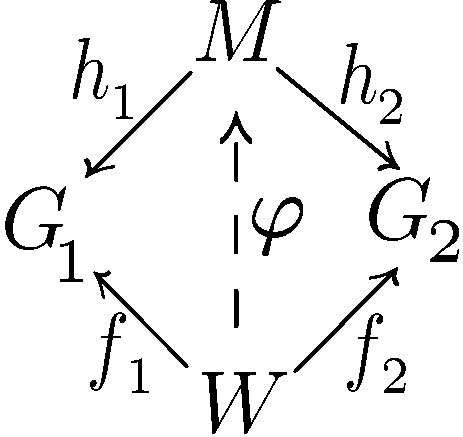
\includegraphics[scale = 0.3]{question9_1.pdf}
\end{thm}

\begin{thm}
  Приведенное выше свойство может быть принято за определение прямого произведения с точностью до изоморфизма.
\end{thm}





\section{Коммутативные кольца. Гомоморфизмы колец. Моно- и эпиморфизмы. Характеризация мономорфизмов.}

\begin{defn}
Кольцом ${A, +, \ast}$ называется множество с 2-мя бин. операциям: $+: A \times A \rightarrow A$ и
$\ast: A \times A \rightarrow A$ и удовлетворяющее следующим условиям:
\begin{enumerate}
 \item $\{A, +\}$ - Абелева группа.
 \begin{enumerate}
  \item $a + b = b + a$
  \item $(a + b) + c = a + (b + c)$
  \item $\exists0: a + 0 = a$
  \item $\forall a \exists -a: a + (-a) = 0$
 \end{enumerate}

 \item $(ab)c = a(bc)$ \\ $\exists e: ea = ae = a$
 \item * $ab = ba$ (коммутативное кольцо)
 \item $a(b+c) = ab + ac$
\end{enumerate}
\end{defn}

Пример: $Z/nZ$ - коммутативное кольцо, $M_n(Z)$ - некоммутативное кольцо.

\begin{defn}
$A, B$ - кольца.\\
$f: A \rightarrow B$ - гомоморфизм колец, если:
\begin{enumerate}
 \item $f(a \ast b) = f(a) \ast f(b)$
 \item $f(a + b) = f(a) + f(b)$
 \item $f(0_A) = 0_B$
 \item $f(1_A) = 1_B$
\end{enumerate}

\begin{flushleft}
Инъективный гомоморфизм - мономорфизм. \\
Сюрьективный гомоморфизм - эпиморфизм. \\
Биективный гомоморфизм - изоморфизм.
\end{flushleft}
\end{defn}

Мы будем рассматривать коммутативные кольца!

\begin{thm}
$ \phi $ - мономорфизм $ \Leftrightarrow ker \phi = \{0\} $
\end{thm}
\begin{proof}
  $ [\Rightarrow] $ Пусть $ \exists a \ne 0 $ $ \phi(a) = 0 $. Но $ \phi(0) = 0 $. Таким образом $ a \ne 0, \phi(a) = \phi(0) $. 
  Противоречие инъективности. \newline
  $ [\Leftarrow] $ Пусть $ \exists a \ne b, \phi(a) = \phi(b) $. Тогда $ \phi(a) - \phi(b) = 0 $,
  а это значит, что $ a - b \ne 0 $ и $ a - b \in ker \phi $. Противоречие тривиальности ядра. 
\end{proof}

\begin{defn}
$f$ - гомоморфизм колец.\\
$Ker(f) = \{a \in A| f(a) = 0_B\}$ - ядро гомоморфизма.
\end{defn}

Свойства ядра:
\begin{enumerate}
 \item $a_1, a_2 \in Ker(f) \Rightarrow a_1 + a_2 \in Ker(f)$
 \item $0_A \in Ker(f)$
 \item $a \in Ker(f), b \in A \Rightarrow ba \in Ker(f)~\&~ab \in Ker(f)$
\end{enumerate}


\section{Идеалы и факторкольца. Определение простого и максимального идеала.}

\begin{defn}
$A$ - кольцо; $\ae \subset A$ \\
$\ae$ - идеал, если:
\begin{enumerate}
 \item $\ae$ - абелева подгруппа\\ $\ae + \ae = \ae, -\ae = \ae$
 \item $A \cdot \ae \subset \ae; \forall c \in A, a \in \ae \Rightarrow ca \in \ae$
\end{enumerate}

\end{defn}

Ядра гомоморфизмов (см. пред. вопрос) колец - идеалы.

Введем отношение эквивалентности на $A$:
\begin{center}
$a_1 \sim a_2 ~ (a_1 \equiv a_2 \mod \ae)~{\buildrel{def}\over{\Leftrightarrow}}~a_1 - a_2 \in \ae$
\end{center}

Будем обозначать: $\overline{a}$ - класс эквивалентности. $\overline{a} = a + \ae$. $\overline{0} = \ae$.

Пусть $\ae$ - идеал в $A$. Построим факторкольцо $A/\ae$ следующим образом. Рассматривая $A$ и $\ae$ как аддитивные группы,
образуем факторгруппу $A/\ae$. Определим теперь в $A/\ae$ умножение: $\overline{a} \cdot \overline{b} = \overline{ab}$.
Проверим, что такое умножение является правильным, т.е. $\overline{a_1} = \overline{a}~\&~\overline{b_1} = \overline{b}
\Rightarrow \overline{a_1b_1} = \overline{ab}$.
\begin{proof}
Нужно показать, что если $a_1 \sim a$ и $b_1 \sim b$, то $a_1b_1 \sim ab$.
\begin{center}
$a_1 = a + a_2, ~a_2 \in \ae$\\
$b_1 = b + b_2, ~b_2 \in \ae$\\

$a_1b_1 = (a + a_2)(b + b_2) = ab + a_2b+b_2a+a_2b_2$\\
$a_1b_1 - ab = a_2b+b_2a+a_2b_2 \in \ae$\\
$a_1b_1 \sim ab$ 
\end{center}
\end{proof}

Таким образом, имеем факторкольцо $A/\ae$.

\begin{thm}
$\phi: A \rightarrow A/\ae$ \\
$\phi(a) = \overline{a};~\phi(ab) = \phi(a)\phi(b)$ \\
$\phi$ - канонический гомоморфизм колец. $Ker(\phi) = \ae$
\end{thm}

\begin{thm}
Ядра гомоморфизмов и только они являются идеалами.
\end{thm}

\begin{defn}
Идеал $\wp \subset A$ называется простым, если: $a_1a_2 \in \wp \Rightarrow (a_1 \in \wp)\vee(a_2 \in \wp)$
\end{defn}

\begin{defn}
Идеал $M \subset A$ называется максимальным, если: $M \neq A$ и если $\beta \supset M$ и $\beta$ - идеал, то $\beta = A$.
\end{defn}

\section{Поля и области целостности. Характеризация простого и максимального идеалов в терминах факторкольца.}

\begin{defn}
Кольцо называтся областью целостности, если в нем нет делителей нуля:
\[\forall x \neq 0, y \neq 0 \Rightarrow xy \neq 0\]
\end{defn}

Пример: $Z$ - область целостности.

\begin{defn}
Поле - кольцо, в котором:
\[\forall x \in A, x \neq 0~~~\exists x^{-1}: xx^{-1} = 1\]
\end{defn}

\begin{thm}
Идеал $\Id{P}$ прост тогда и только тогда, когда $A/\Id{P}$ - область целостности
\end{thm}
\begin{proof}
$[\Rightarrow]$ $\Id{P}$ прост.
\[\overline{0} \neq \overline{x} \in A/\Id{P}\]
\[\overline{0} \neq \overline{y} \in A/\Id{P}\]
Покажем, что $\overline{x} \cdot \overline{y} \neq \overline{0}$.
\[x \notin \Id{P}, y \notin \Id{P} \Rightarrow xy \notin \Id{P} \Leftrightarrow \overline{xy} \neq \overline{0}
\Leftrightarrow \overline{x}\cdot\overline{y} \neq \overline{0}\]
$[\Leftarrow]$ $A/\Id{P}$ - область целостности. Пусть $\Id{P}$ - не прост. Тогда $\exists a_1, a_2: a_1a_2 \in \Id{P}$,
но $a_1 \notin \Id{P}~\&~a_2 \notin \Id{P}$. Рассмотрим соответствующие классы эквивалентности:
\[\overline{a_1} \neq \overline{0}~\&~\overline{a_2} \neq \overline{0} \]
\[\overline{a_1a_2} = \overline{a_1}\cdot\overline{a_2} = \overline{0}\]
Но $A/\Id{P}$ - область целостности. Получили противоречие.
\end{proof}

ЗАМЕЧАНИЕ: $1 \in \Id{B} \Leftrightarrow \Id{B} = A$.

\begin{defn}
$S \subset A$, тогда $(S)$ - идеал, порожденный множеством $S$, т.е. пересечение всех идеалов, содержащих $S$.
\end{defn}


\begin{thm}
$\Id{M}$ - максимальный $\Leftrightarrow$ $A/\Id{M}$ - поле
\end{thm}
\begin{proof}
$[\Rightarrow]$ $\Id{M}$ - максимальный идеал. Покажем, что $A/\Id{M}$ - поле. Возьмем ненулевой элемент и найдем обратный
к нему.
\[\overline{x} \in A/\Id{M},~~~\overline{x} \neq \overline{0} \Leftrightarrow x \notin \Id{M}\]
\[(\Id{M}\bigcup\{x\}) = A \Rightarrow 1 \in (\Id{M}\bigcup\{x\})\]
\[(\Id{M}\bigcup\{x\}) = xA + \Id{M}\]
\[\exists y \in A, ~ m_1 \in \Id{M}: 1 = xy + m_1 \Leftrightarrow \overline{1} = \overline{x}\cdot\overline{y} + \overline{0}
 = \overline{xy}
\]
$[\Leftarrow]$ $A/\Id{M}$ - поле. Пусть $\Id{M}$ не максимальный. Тогда $\exists \Id{M}_1: \Id{M} \subset \Id{M}_1
\subset A$. Возьмем $x \in \Id{M}_1\setminus\Id{M}$:
\[(\Id{M}\bigcup\{x\}) \subset \Id{M_1} \Rightarrow 1 \notin (\Id{M}\bigcup\{x\})\]
Рассмотрим $\overline{x} \in A/\Id{M}$. Т.к. $A/\Id{M}$ - поле, то $\exists \overline{y} \in A/\Id{M}:~
\overline{x}\cdot\overline{y} = \overline{1}.$
\[\exists m_1, m_2 \in \Id{M}: (x + m_1)(y + m_2) = 1 = xy + m_1y + m_2x + m_1m_2 = 1 \Rightarrow 1 \in
(\Id{M}\bigcup\{x\})\]
Получили противоречие.
\end{proof}

\begin{thm}
Максимальный идеал простой.
\end{thm}
\begin{proof}
Пусть $\Id{M}$ - максимальный идеал, и пусть $x, y \in A$ таковы, что $xy \in \Id{M}$. Предположим, что $x \notin \Id{M}$.
Тогда $\Id{M} + Ax$ - идеал, строго содержащий $\Id{M}$ и,  стало быть, равный $A$. Следовательно, мы можем написать
\[1 = u + ax,\] где $u \in \Id{M}$ и $a \in A$. Умножая на $y$, получаем $y = yu + axy$, откуда $y \in \Id{M}$ и $\Id{M}$,
таким образом, простой. 
\end{proof}
\end{document}

